\documentclass[12pt, a4paper]{article}

\usepackage{listings}
\usepackage{color}
\usepackage{enumitem}
\usepackage{amsthm}
\usepackage{amssymb}
\usepackage{listings}
\usepackage{setspace}
\usepackage{relsize}
\usepackage{graphicx}
\graphicspath{ {./figures/} }


\title{General Physics: Mechanics, Heat, and Sound}
\author{William Darko}
\date{Fall 2021}

\pagenumbering{arabic}

\begin{document}

\maketitle
\newpage

\tableofcontents

\newpage

\section{Kinematics in 1D}
\paragraph*{}
Kinematics in 1 dimension refers to the motion of objects, on \textbf{1 spatial dimension},
not necessarily in a one dimensional space. One can still observe 1 dimensional
kinematics of objects in multidimensional spaces.

\subsection{Reference Frames}
\paragraph*{}
Measurements of \textbf{position, distance, speed} must be with respect to 
a \textbf{reference frame}.

\subsection{Displacement and Distance}

\subsubsection{Displacement}
\paragraph*{}
\textbf{Displacement} is the measure of \textbf{how far an object is from its initial (starting)
position, and its final postion}. Measure of displacement isn't dependant on the actual path
taken by the object, or the length of that path, all that matters is the starting position, and finishing position.

Displacement is defined as:

{
    \centering
    $\Delta x = x_2 - x_1$

}
where $x_2$ and $x_1$ are the final, and initial positions of the object, respectively. Displacement
is represented as a vector; a quantity with a \textbf{magnitude, and direction}.

\subsubsection{Distance}
\paragraph*{}
There's a difference between displacement, and distance. While displacement is 
only concerned with the absolute difference between the initial and final position of an object,
\textbf{distance} is concerned about the \textbf{absolute length of the path taken by the object}.
Distance is \textbf{represented as a scalar quantity}.


\subsection{Average Velocity, and Speed}

\subsubsection{Average Speed}
\paragraph*{}
\textbf{Defined as:}

{
    \centering
    \textbf{avg speed =} $\frac{\textrm{
        \textbf{\textit{distance travelled}}}}{\textrm{\textbf{\textit{time elapsed}}}}$ = $\frac{\textbf{d}}{\textbf{$\Delta t$}}$

}

\subsubsection{Average Velocity}
\paragraph*{}
Velocity is the change in rate of change in position, thus we're concerned with 
directional information; in what direction is our object moving. Thus average velocity 
is defined as:

{
    \centering
    \textbf{avg velocity =} $\frac{\textbf{\textit{displacement}}}{\textrm{\textbf{\textit{time elapsed}}}}$ = 
    {$\frac{\textbf{$\Delta x$}}{\textbf{$\Delta t$}}$}

}

\subsubsection{Instantaneous Velocity}
\paragraph*{}
Instantaneous velocity is the \textbf{average velocity as the time elapsed becomes infinitely small}.
In other words, as the limit of average velocity as time elapsed approaches 0:

{
    \centering
    \textbf{\textit{v} = } $\textrm{\textbf{\textit{lim}}}_{\textrm{$\Delta t \rightarrow 0$}}$ 
    \textbf{${\frac{\textrm{$\Delta x$}}{\textrm{$\Delta t$}}}$}

}

\subsection{Acceleration}
\paragraph*{}
Acceleration of an object is the \textbf{rate of change of that objects velocity}. Mathematically:

{
    \centering
    \textbf{avg acceleration =} $\frac{\textbf{\textit{ROC of velocity}}}{\textrm{\textbf{\textit{time elapsed}}}}$ = 
    \textbf{${\frac{\textrm{$\Delta v$}}{\textrm{$\Delta t$}}}$}

} 

\paragraph*{}
acceleration is also a vector quantity. In a single spatial dimension we really only care about
the sign. 

\textbf{Negative acceleration} is acceleration in the negative direction as defined by the spatial coordinate system.

\textbf{Deceleration} occurs when acceleration is opposite in direction to velocity.

\textbf{Instantaneous acceleration} is the average acceleration as the time elapsed becomes infinitely small.
In other words, the limit of average velocity as the time interval approaches 0. 

{
    \centering
    \textbf{\textit{a } = } $\textrm{\textbf{\textit{lim}}}_{\textrm{$\Delta t \rightarrow 0$}}$ 
    \textbf{${\frac{\textrm{$\Delta v$}}{\textrm{$\Delta t$}}}$}

}
\newpage

\subsection{Motion at constant acceleration}
\paragraph*{}
We know the average volocity of an object during a time interval \textbf{\textit{t}} is:

{
    \centering
    $\mathlarger{\bar v = \frac{\Delta x}{\Delta t} = \frac{x_1 - x_0}{t_1 - t_0} = \frac{x_1 - x_0}{t}}$

}
\paragraph*{}
in other words, ratio of displacement, to time elapsed. We also know that acceleration, assumed constant, is:

{
    \centering
    $ \mathlarger{a = \frac{v_1 - v_0}{t}}$

}
where $v_1$, $v_0$, and $t$ are observed velocities and time elapsed, respectively. In other words,
the acceleration when constant is the difference/change in two observed velocites, divided by the observed elapsed time.

We also know that the average of any two numerical quantities is the sum of them divided by two. Thus, we can observe that the
average velocity can be defined as:

{
    \centering
    $\mathlarger{\bar v = \frac{v_1 + v_0}{2}}$

}

\paragraph*{}
Now, combining the last three equations, we can see that the equation for the postion \textbf{\textit{x}} of a particle
in rectilinear space is the initial position $x_0$ plus the average rate of change of position (average velocity) over a certain time period.
Thus:

{
    \centering
    $\mathlarger{x = x_0 + \bar vt}$

    $\mathlarger{x = x_0 + (\frac{v_0 + v_1}{2})t}$

    $\mathlarger{x = x_0 + (\frac{v_0 + v_0 + at}{2})}$

    $\therefore$ $\mathlarger{x = x_0 + v_0t + \frac{1}{2}at^2}$

    to get rid of $t$, we combine the equations to get:

    $\mathlarger{v^2 = v_0^2 + 2a(x-x_0)}$

}

\paragraph*{}
We can now solve any constant acceleration problem with the following equations:

{
    \centering
    $\mathlarger{v = v_0 + at}$

    $\mathlarger{x = x_0 + v_0t + \frac{1}{2}at^2}$

    $\mathlarger{v^2 = v_0^2 + 2a(x-x_0)}$

    $\mathlarger{\bar v = \frac{v_1 + v_0}{2}}$

}

\subsection{Falling objects}
\paragraph*{}
Near the earth's surface, all objects experience approximately the same acceleration
due to the force of gravity; thus expereince motion with constant acceleration.

In the absence of air resistance, like in a vacuum, objects fall with the same  acceleration.

Acceleration due to earths gravity is approximately \textbf{\textit{g = 9.8 $m/s^2$}}

With gravity introduced, all the equations we've developed for constant acceleration still hold; as 
we observe linear motion on the \textbf{proper spatial \textit{y-axis}}, our equations become:

{
    \centering
    $\mathlarger{v_y = v_{y0} + a_yt}$

    $\mathlarger{y = y_0 + v_{y0}t + \frac{1}{2}a_yt^2}$

    $\mathlarger{v_y^2 = v_{y0}^2 + 2a(y-y_0)}$

    $\mathlarger{\bar v_y = \frac{v_{y1} + v_{y0}}{2}}$

}

where the \textbf{\textit{y}} subscript represents the quantities observed on the spatial \textbf{\textit{y-axis}}. Thus,
our acceleration $\textrm{\textbf{a}}_\textrm{\textbf{\textit{y}}}$ here since we're observing free falling objects along the spatial \textbf{\textit{y-axis}}
is:

{
    \centering
    $\textrm{\textbf{a}}_\textrm{\textbf{\textit{y}}} = \textrm{\textbf{9.8
    \textit{m/s}}}^\textrm{\textbf{2}}$

}

and negative, if moving in the negative direction along the coordinate system, as per the defintion of
negative acceleration.


\newpage

\section{Kinematics in 2-Dimensions, and Vectors}

\subsection{Vectors and Scalars}
\paragraph*{}
Vectors are quantities that have a \textbf{magnitude, and a direction} as well. Scalars on the other hand
have \textbf{only a magnitude}. Vectors are usually represented as n-tuples in some vector space 
$\mathbb{R} ^n$, while scalars are numerical values like 2, 5, $\alpha$, etc.

Examples of some vector quantities: \textbf{displacement, velocity, force, momentum}. Examples of scalar quantities:
\textbf{mass, time, temperature}.

\subsection{Addition of vectors (graphical interpretation)}
\paragraph*{}
Geometrically, vector addition, suppose we were to add vectors $V + W$, comprises of 
placing the tail of vector $W$ at the head of vector $V$: \\

{
    \centering
    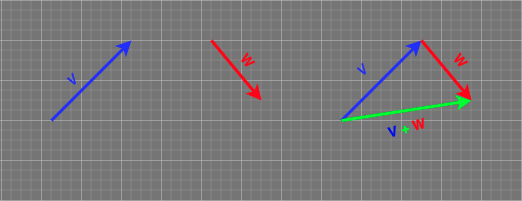
\includegraphics[width=12cm]{phys_vector_add_geom.png}

}

\paragraph*{}
Displacement can be found also using vectors, by employing the pythagorean
theorem. Suppose vectors $V$ and $W$ are orthogonal, thus form a $90$ degree angle,
then we can find vector $P = V + W$ by doing:

{
    \centering
    $\mathlarger{P = \sqrt{V^2 + W^2}}$

}

\paragraph*{}
We can also use trigonometric functions to find the other angles in the triangle. For example,
the anlge $\theta$ between vector $V$ and $P$ can be found using:

{
    \centering
    $\mathlarger{tan \theta = \frac{W}{P}}$

}

\newpage
\subsection{Vector subtraction and scalar multiplication}
\paragraph*{}
Vector subtraction of two vectors $V$, $W$ can be found can be computed via component wise
substraction, or by geometric interpretation: \\

{
    \centering
    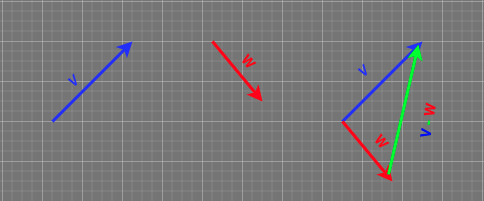
\includegraphics[width=12cm]{phys_vec_sub.png}

}


\subsection{Algebraic formulae for computing vectors}

\paragraph*{}

{
    \centering
    $\mathlarger{v_x=vcos\theta}$\textbf{,} $\mathlarger{v_y=vsin\theta}$

    $\mathlarger{v = \sqrt{v_x^2 + v_y^2}}$\textbf{,} $\mathlarger{tan\theta=\frac{v_y}{v_x}}$

    $\mathlarger{sin(90-\theta) = cos\theta}$\textbf{,} $\mathlarger{cos(90-\theta) = sin\theta}$

}

\paragraph*{}
Steps for computing geometrically/algebraically:
\begin{enumerate}
    \item Draw diagram originating each vector from the originating
    \item Choose $x$ and $y$ axes
    \item Write vectors as their components
    \item Compute components and add them in appropriate direction
    \item Calculate magnitude, and direction of resulting vector
\end{enumerate}


\newpage
\subsection{Projectile Motion}

\paragraph*{}
A projectile is an \textbf{object moving in along 2 spatial dimensions} (not necessarily in 2 dimensional space)
\textbf{under the influence of Earth's gravity}. Its path near the surface of the Earth resembles 
a parabola.


\end{document}